%%% ======= Beamer ======
\documentclass[usenames,dvipsnames,t]{beamer}
% \documentclass[usenames,dvipsnames, handout]{beamer}
\beamertemplatenavigationsymbolsempty % remove toolbar at the bottom of slides
\usepackage{appendixnumberbeamer} % for appendix
\usetheme{Madrid}
\usecolortheme{default}
\useinnertheme{circles}

\usepackage[style=numeric-comp,sorting=none,backend=biber]{biblatex}%<- specify style
\addbibresource{references.bib}%<- specify bib file


\setbeamercolor{author in head/foot}{bg=blue!10, fg=blue}
\setbeamercolor{title in head/foot}{bg=blue!10, fg=blue}
\setbeamercolor{date in head/foot}{bg=blue!10, fg=blue}

\makeatletter
\setbeamertemplate{footline}{
  \leavevmode%
  \hbox{%
  \begin{beamercolorbox}[wd=.333333\paperwidth,ht=2.25ex,dp=1ex,center]{author in head/foot}%
    \usebeamerfont{author in head/foot}\insertshortauthor\expandafter\ifblank\expandafter{\beamer@shortinstitute}{}{~~(\insertshortinstitute)}
  \end{beamercolorbox}%
  \begin{beamercolorbox}[wd=.333333\paperwidth,ht=2.25ex,dp=1ex,center]{title in head/foot}%
    \usebeamerfont{title in head/foot}\insertshorttitle
  \end{beamercolorbox}%
  \begin{beamercolorbox}[wd=.333333\paperwidth,ht=2.25ex,dp=1ex,right]{date in head/foot}%
    \usebeamerfont{date in head/foot}\insertshortdate{}\hspace*{2em}
    \insertframenumber{}%
%     / \inserttotalframenumber
    \hspace*{2ex} 
  \end{beamercolorbox}}%
  \vskip0pt%
}
\makeatother

\colorlet{beamer@blendedblue}{blue!70} % change color theme


% For appendix
\newcommand{\backupbegin}{
   \newcounter{framenumberappendix}
   \setcounter{framenumberappendix}{\value{framenumber}}
}
\newcommand{\backupend}{
   \addtocounter{framenumberappendix}{-\value{framenumber}}
   \addtocounter{framenumber}{\value{framenumberappendix}} 
}

\setbeamertemplate{bibliography item}{\insertbiblabel} % improved references



% Other preamble stuff:
\usepackage{preamble}

%%% Uncomment for another color palette
% \definecolor{Logo1}{rgb}{0.0, 0, 0.7}
% \definecolor{Logo2}{rgb}{2.55, 2.55, 2.55}

% \setbeamercolor*{palette primary}{bg=Logo1, fg=white}
% \setbeamercolor*{palette secondary}{bg=Logo2, fg=white}
% \setbeamercolor*{palette tertiary}{bg=white, fg=Logo1}
% \setbeamercolor*{palette quaternary}{bg=white,fg=white}
% \setbeamercolor{structure}{fg=Logo1} % itemize, enumerate, etc
% \setbeamercolor{section in toc}{fg=Logo1} % TOC sections

% For figures
\usepackage{import}
\usepackage{xifthen}
\usepackage{pdfpages}
\usepackage{transparent}
\usepackage{mdframed}

% --- Inkscape figures:
\newcommand{\incfig}[2][0.75\textwidth]{%
    \def\svgwidth{\columnwidth}
    \resizebox{#1}{!}{\import{Inkscape figs/}{#2.pdf_tex}}
}

% --- Height of frame
\newlength{\myheight}
\setlength{\myheight}{7cm}


%------------------------------------------------------------
%This block of code defines the information to appear in the
%Title page
\title[QCD JC] %optional
{Kilonovae}

\author{Thibeau Wouters}

\date{March 5, 2024}




%End of title page configuration block
%------------------------------------------------------------



%------------------------------------------------------------
%The next block of commands puts the table of contents at the 
%beginning of each section and highlights the current section:

\AtBeginSection[]
{
  \begin{frame}[plain, noframenumbering]
    \frametitle{Table of Contents}
    \tableofcontents[currentsection]
  \end{frame}
}

\AtBeginSubsection[]
{
  \begin{frame}[plain, noframenumbering]
    \frametitle{Table of Contents}
    \tableofcontents[currentsection]
  \end{frame}
}


%------------------------------------------------------------


\begin{document}

% {

% \usebackgroundtemplate{\transparent{0.30}{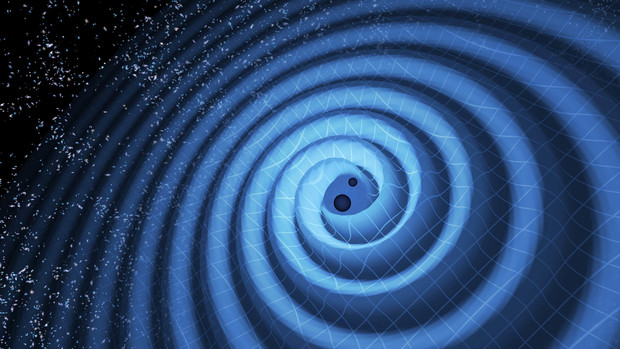
\includegraphics[width=\paperwidth,height=\paperheight]{Figures/GW-2.jpeg}}}


% \begin{frame}[plain]
% \titlepage

% % \begin{figure}
% % \centering
% % 
\includegraphics[width=0.25\textwidth]{Figures/utrecht-university.png}
% % \end{figure}

% \end{frame}
% }

\begin{frame}[plain]
\titlepage
\end{frame}

% %The next statement creates the title page.
% \frame[plain]{\titlepage



% }


%---------------------------------------------------------
%This block of code is for the table of contents after
%the title page
\begin{frame}[plain, noframenumbering]
\frametitle{Table of Contents}
\tableofcontents
\end{frame}
%---------------------------------------------------------


\section{Introduction}

\begin{frame}{Multimessenger astrophysics}

  \def\x{5mm}

  \def\y{3mm}

\begin{itemize}
  \item Multimessenger astrophysics: GW + \textbf{EM}: signature of NS-BH or NS-NS mergers
  
  \vspace{\x}
  
  \item Hard: sky localisation from GW is bad 
  
  \vspace{\x}

  \item \href{https://youtu.be/xBvz5ilc8rE?si=75NmXKUTWbuUlOjW}{Excellent video on GW170817, the first multimessenger event}
  \begin{itemize}
    \item $t + 0$ s: GW observed by Hanford, Livingston, Virgo
    
    \vspace{\y}
    
    \item $t + 1.7$ s: Short GRB
    
    \vspace{\y}
    
    \item $t + $ days: kilonova
  \end{itemize}
  
  \vspace{\x}


\end{itemize}

\end{frame}

\begin{frame}{Kilonovae}

  ``\textbf{Kilonovae} are thermal supernova-like transients lasting days to weeks, which are powered by the radioactive decay of heavy neutron-rich elements synthesized in the expanding merger ejecta"~\cite{Metzger:2019zeh}

  \begin{figure}
    \centering
    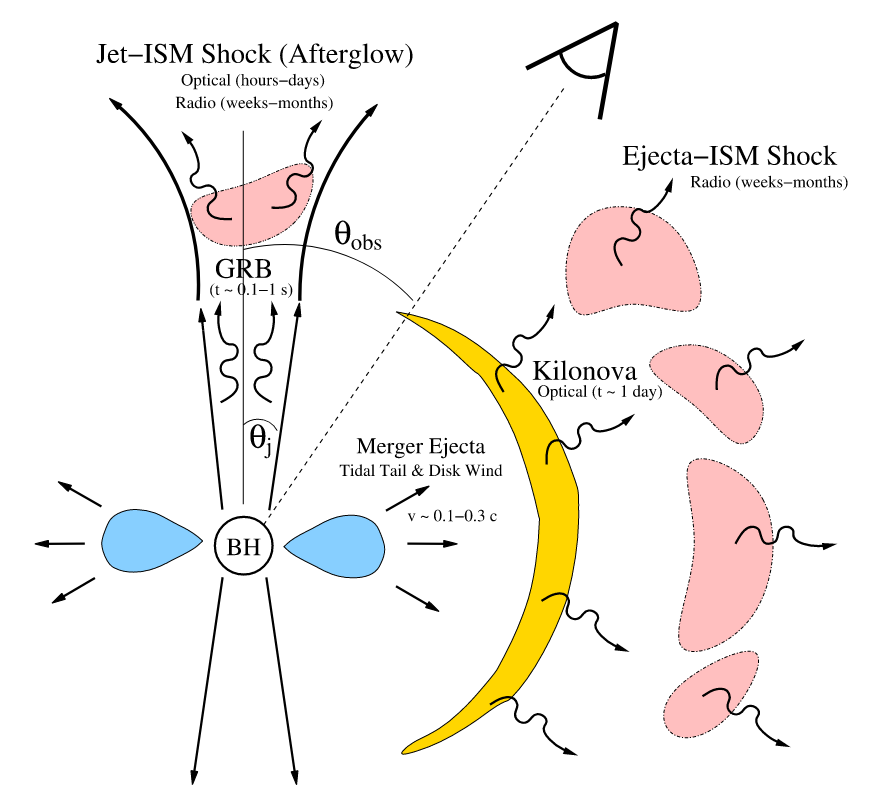
\includegraphics[width=0.5\textwidth]{Figures/EM-counterparts.png}
  \end{figure}
\end{frame}

\begin{frame}{$r$-process}
  \def\x{3mm}

\begin{itemize}
  \item \red{$r$-process}: formation heavy elements, needs neutron-rich environment
  
  \vspace{\x}
  
  \item Depends on electron fraction $Y_e$
  \begin{equation*}
    Y_e = \frac{n_p}{n_p + n_n} \, 
  \end{equation*}
  \begin{itemize}
    \item Ordinary matter: $Y_e > 0.5$
    \item $r$-process: needs $Y_e < 0.5$
  \end{itemize}

  \vspace{\x}
  
  \item NS mergers likely dominant source of $r$-process (?)
\end{itemize}
\end{frame}

\section{General remarks}

\begin{frame}{Basic ingredients}

  \def\x{3mm}
  \def\y{1mm}

  % Peak time, luminosity, effective temperature from 3 ingredients:
  % \vspace{\y}
  % \begin{enumerate}
  %   \item Mass, velocity of ejecta (can be different components)
    
  %   \vspace{\x}
    
  %   \item Opacity of matter
    
  %   \vspace{\x}
    
  %   \item Sources of heating of ejecta
  % \end{enumerate}

  % \pause

  Important are \red{mass} and \red{velocity} of ejecta. Type of ejecta depends on
  \vspace{\y}
  \begin{enumerate}
    \item Scenario (NS-BH vs NS-NS)
    
    \vspace{\x}
    
    \item For NS-NS: mass of NSs and \textbf{EOS quantities} (TOV mass)
  \end{enumerate}

  \begin{figure}
    \centering
    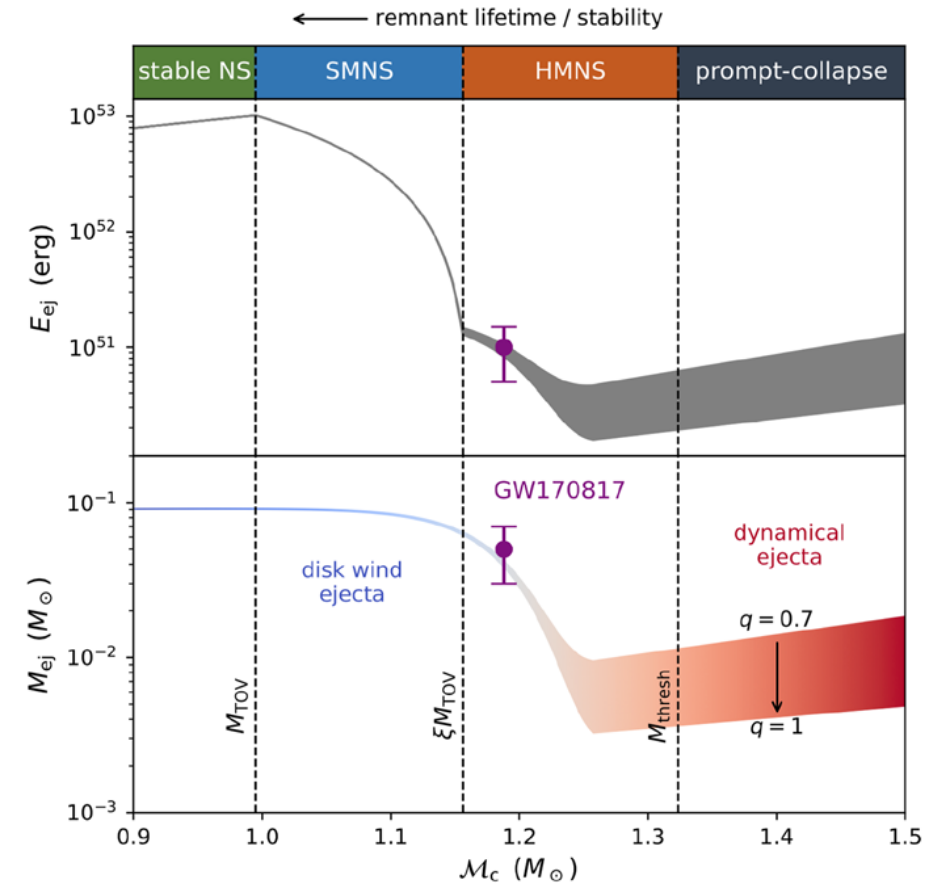
\includegraphics[width=0.5\textwidth]{Figures/mass_ejecta_vs_Mc_NS_lifetimes.png}
  \end{figure}

\end{frame}

\begin{frame}{Red and blue kilonovae}

  \begin{itemize}
    \item \red{Red kilonovae}: low $Y_e$, lanthanide-rich
    
    \vspace{3mm}
    
    \item \blue{Blue kilonovae}: high $Y_e$, no lanthanides
    
    \vspace{3mm}

    \item Longer-lived remnants: higher Ye: bluer kilonovae
  \end{itemize}
  
  \begin{figure}
    \centering
    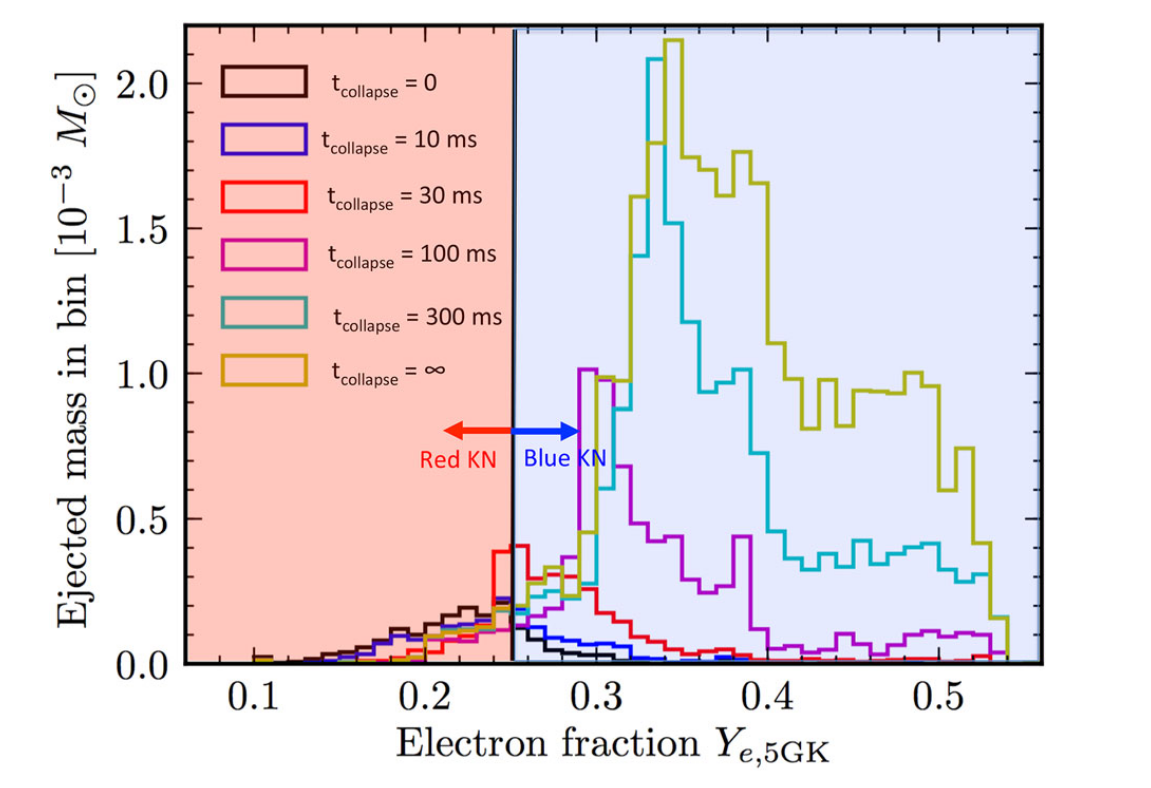
\includegraphics[width=0.7\textwidth]{Figures/lifetime_remnant_and_blue_red_KN.png}
  \end{figure}

\end{frame}

\section{Kilonova models}

\begin{frame}{\texttt{POSSIS}}

  \def\x{2.5mm}

  \texttt{POSSIS}~\cite{Bulla:2019muo}: time-dependent 3D Monte Carlo radiative transfer code


  \begin{itemize}
    \item Monte Carlo packets of photons
    
    \vspace{\x}
    
    \item Packets propagated until interaction with matter
    
    \vspace{\x}
    
    \item Can handle arbitrary geometry for ejecta
    
    \vspace{\x}
    
    \item Time- and wavelength-dependent opacities
    
    \vspace{\x}
    
    \item Synthetic observables: light curves, spectra, polarisation
    
    
  \end{itemize}

  \begin{figure}
    \centering
    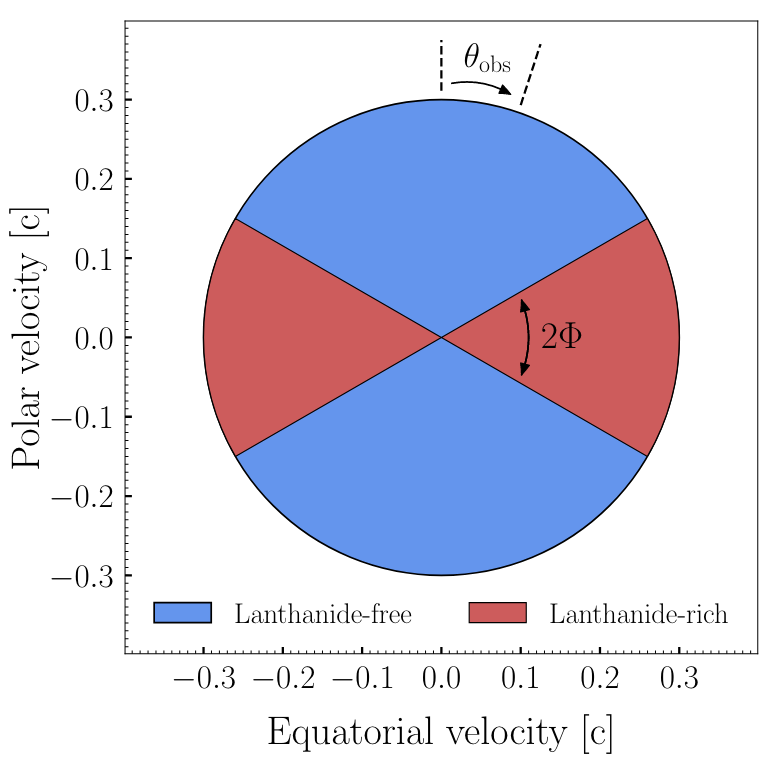
\includegraphics[width=0.325\textwidth]{Figures/bulla_model.png}
  \end{figure}
  
\end{frame}

\begin{frame}{Example light curve}
    Example light curve -- how to use in Bayesian analysis?
    \begin{figure}
      \centering
      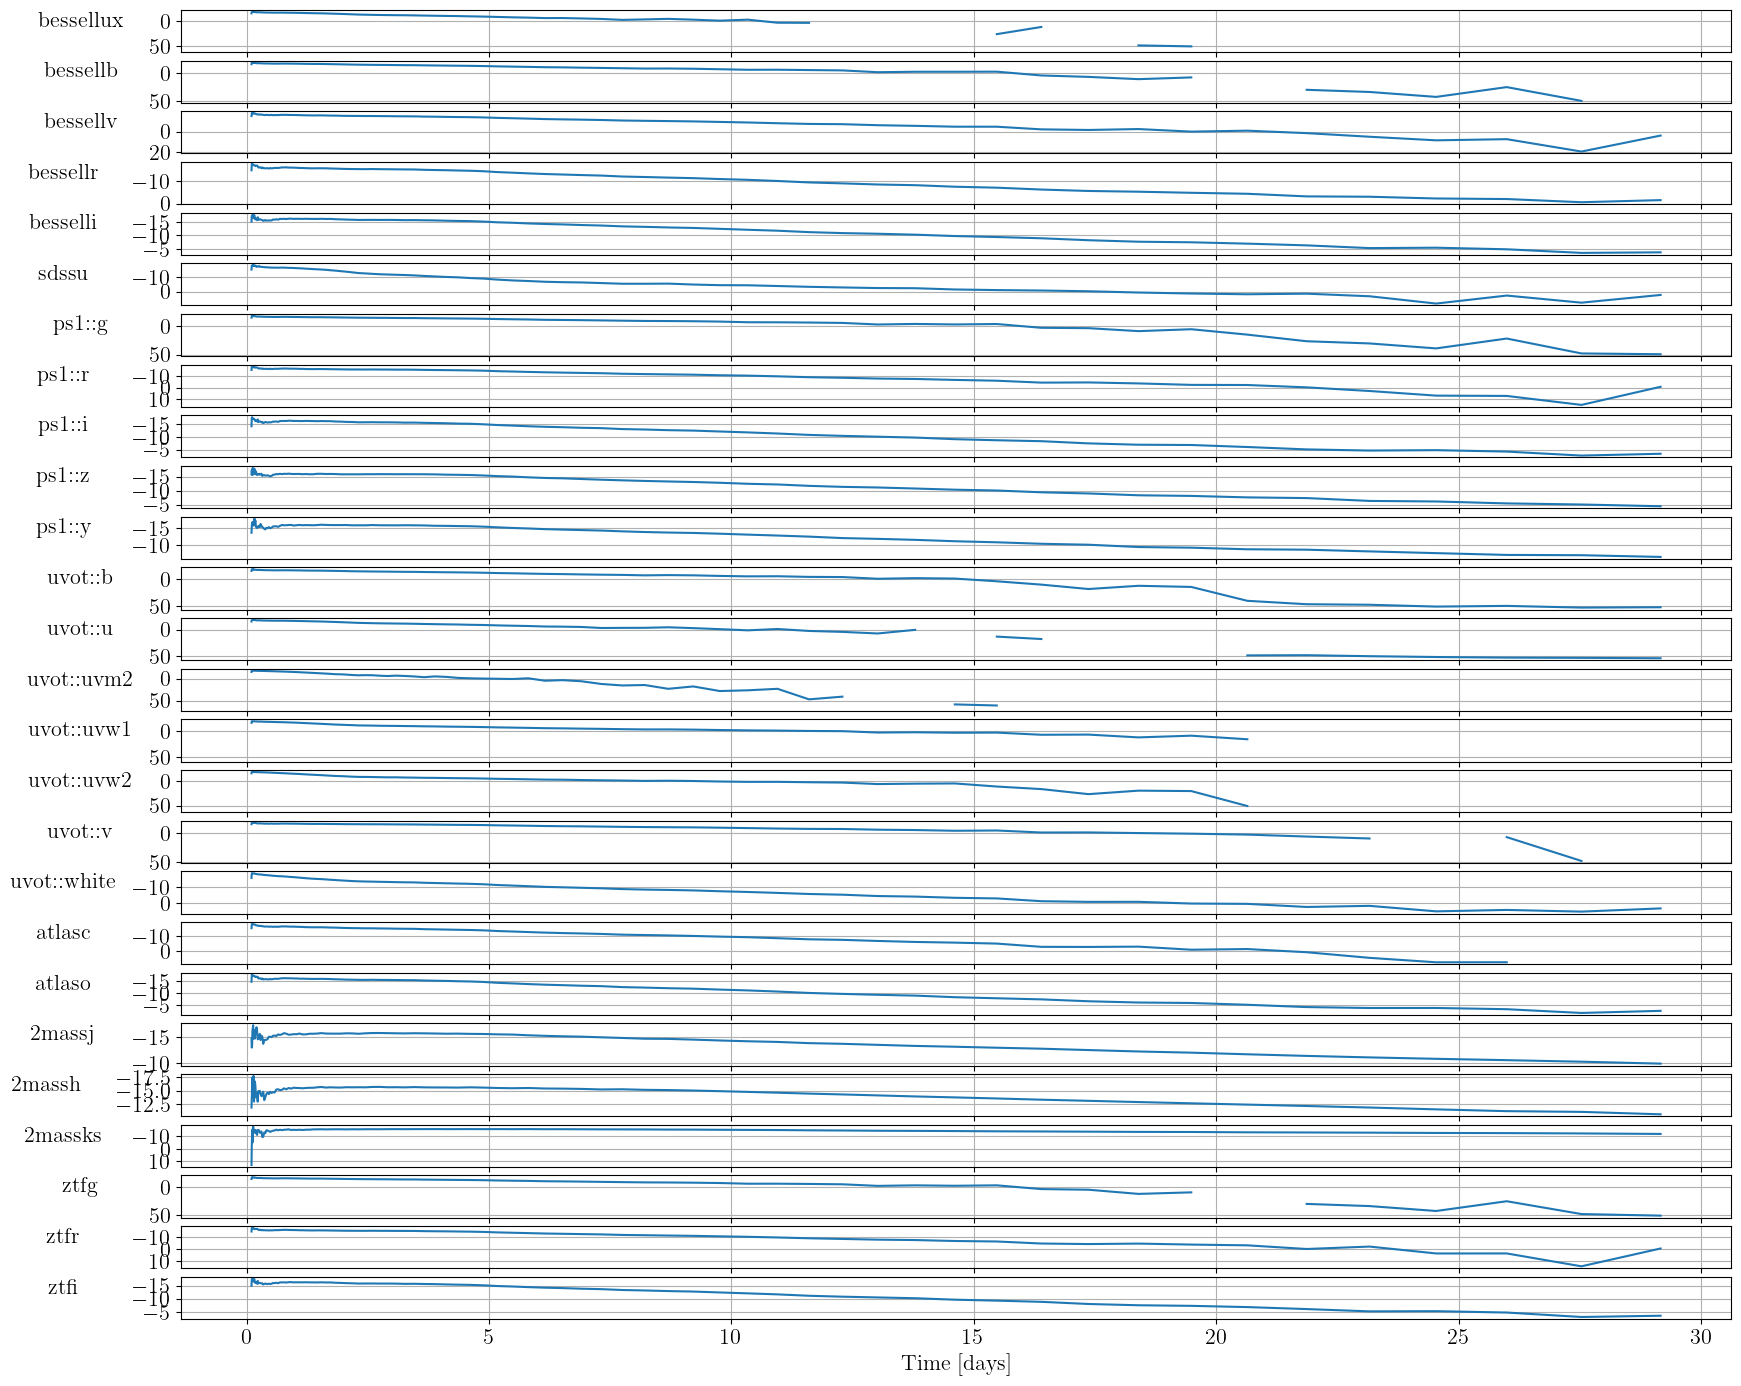
\includegraphics[width=0.75\textwidth]{Figures/example_bulla_LC.png}
    \end{figure}
\end{frame}

\begin{frame}{Surrogate models}

  \def\x{3mm}
  \def\y{2mm}

  Train a surrogate model:
  \begin{enumerate}
    \item Training data: grid of \texttt{POSSIS} light curves: $\left\{ (\theta_{\rm KN}; m_i) \right\}$
    
    \vspace{\x}
    
    \item Reduce dimensionality: SVD: $m_i \mapsto \tilde{m}_i$ ($\R^{100} \to \R^{10}$)
    
    \vspace{\x}
    
    \item Train neural network: NN: $\theta_{\rm KN} \mapsto \tilde{m}_i$

  \end{enumerate}

  \vspace{\y}

  \only<2>{
    \begin{figure}
      \centering
      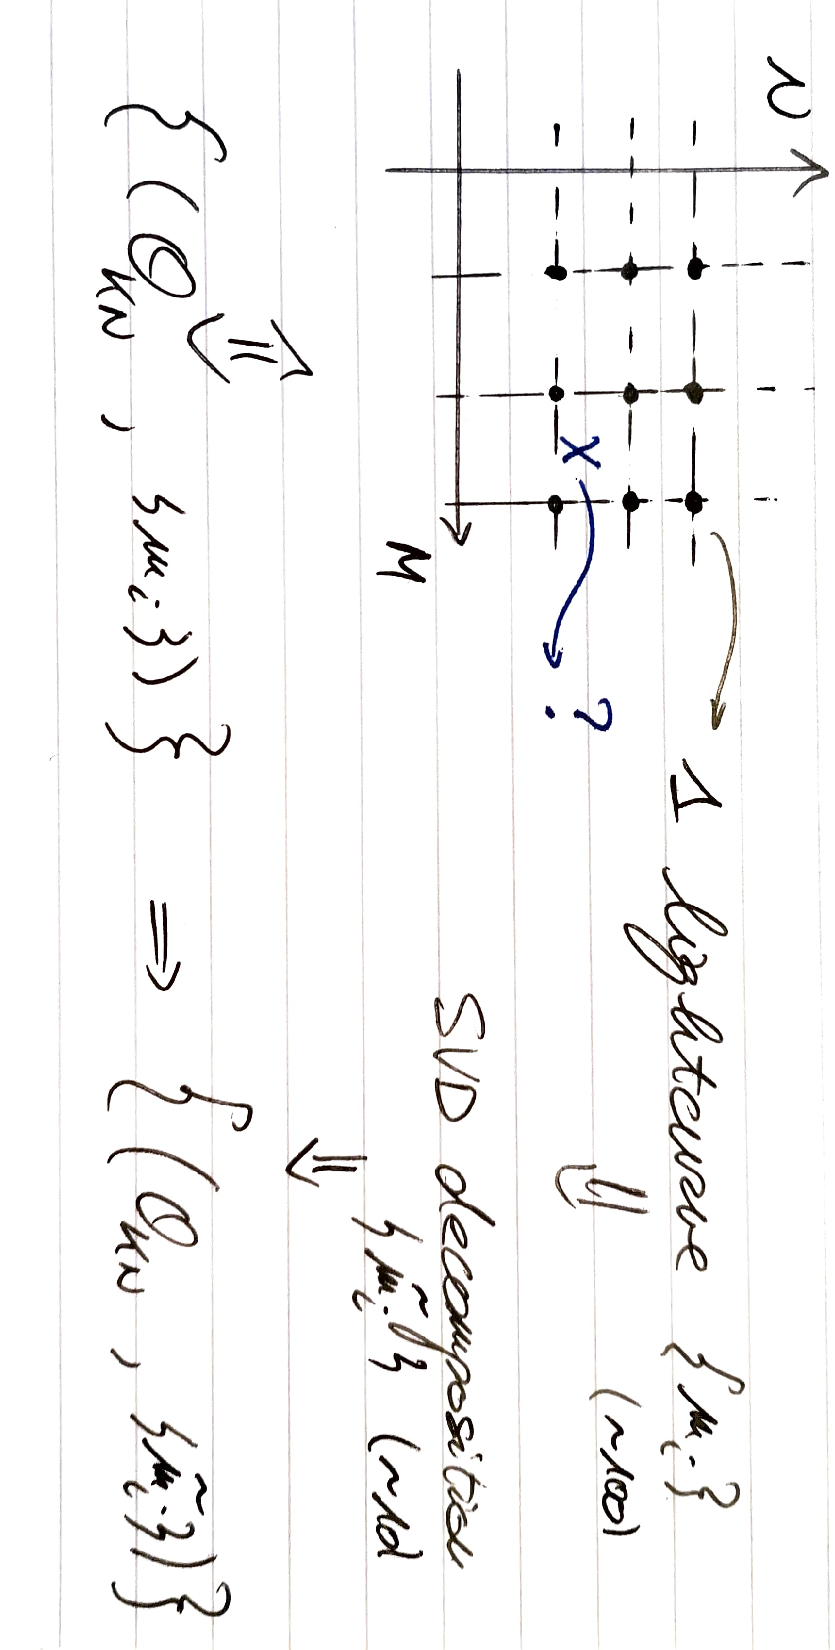
\includegraphics[angle=90, width=0.75\textwidth]{Figures/surrogate_1.pdf}
    \end{figure}
  }

  \only<3>{
    \begin{figure}
      \centering
      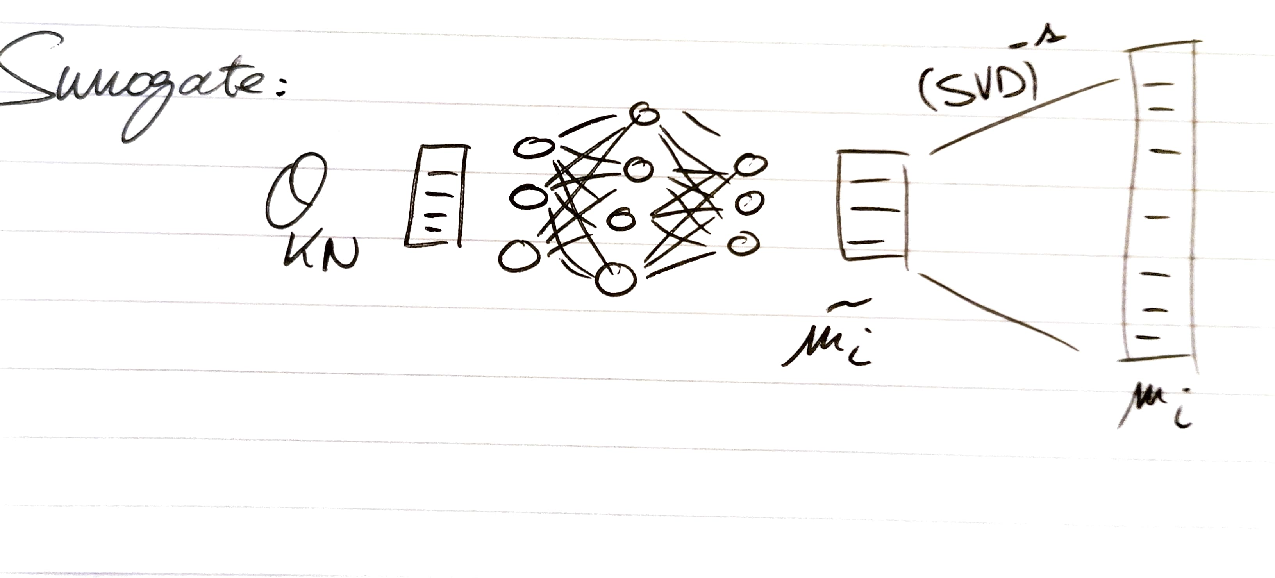
\includegraphics[width=0.75\textwidth]{Figures/surrogate_2.pdf}
    \end{figure}
  }

  \only<4>{
    \begin{figure}
      \centering
      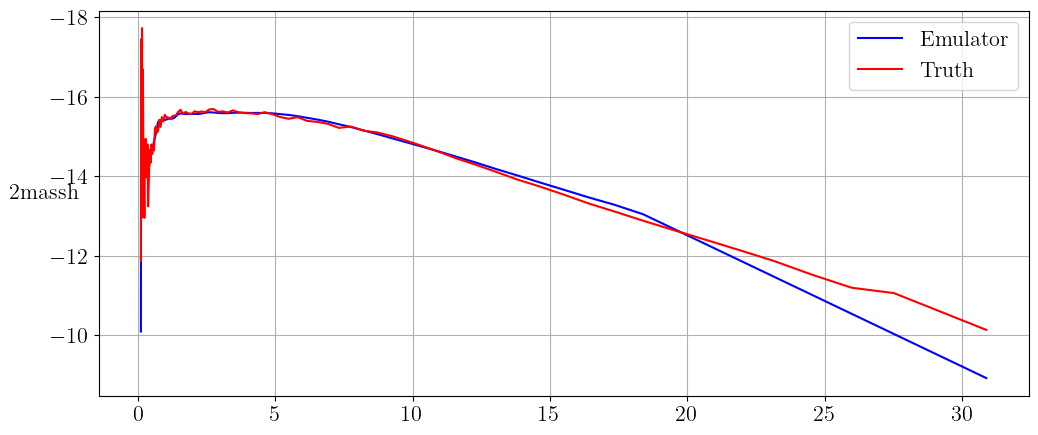
\includegraphics[width=0.75\textwidth]{Figures/example_emulated_LC.png}
    \end{figure}
  }

\end{frame}


\begin{frame}{Example: end result AT2017gfo}
  
  Result from \texttt{NMMA} (with GW and GRB)~\cite{Pang:2022rzc}
  \begin{figure}
    \centering
    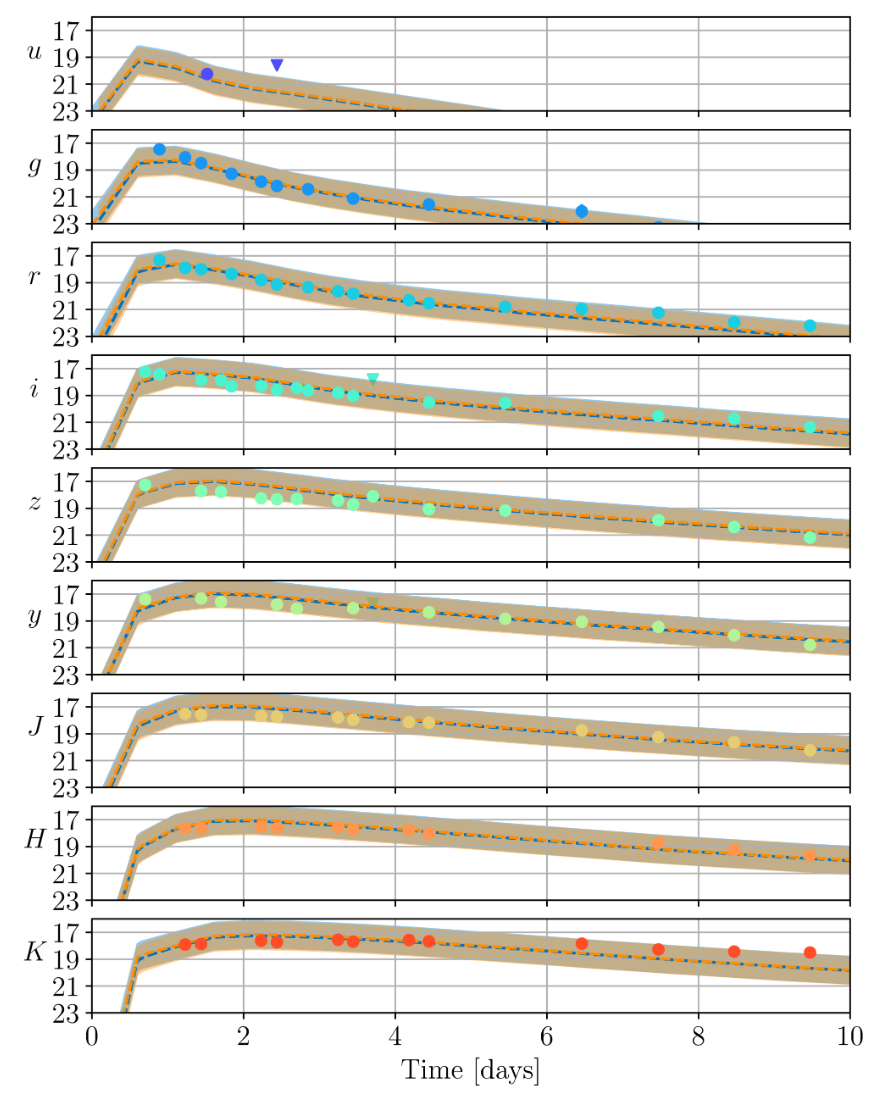
\includegraphics[width=0.475\textwidth]{Figures/NMMA_AT2017gfo.png}
  \end{figure}

\end{frame}


\section{Conclusion and outlook}

\begin{frame}{Conclusion and outlook}

  \def\x{3mm}
  \def\y{7mm}

  Conclusion: 
  \begin{itemize}
    \item Kilonovae: important EM counterpart to GW events, EOS dependent
    
    \vspace{\x}

    \item Important for understanding $r$-process (Jasper next week)
    
    \vspace{\x}

    \item \texttt{POSSIS} and surrogate models: tools to model kilonovae
  \end{itemize}


  \vspace{\y}

  Outlook:
  \begin{itemize}
    \item Bayesian analysis over KN models
    
    \vspace{\x}

    \item GRB counterparts
    
    \vspace{\x}

    \item Joint inference over GW \& EM (KN + GRB)
    
    \vspace{\x}

    \item EOS constraints from GW170817
    
    % \vspace{\x}

    % \item Surrogate models: improved architecture
  \end{itemize}  
  
\end{frame}


\begin{frame}{References}
  
  \printbibliography

\end{frame}

\end{document}

